    \documentclass{minimal}
     
    %dvipdfmx
    \usepackage[dvipdfmx]{animate}
    \def\pgfsysdriver{pgfsys-dvipdfmx.def}
     
    %pdftex or latex+dvips
    %\usepackage{animate}
     
    \usepackage{tikz}
     
    \begin{document}
     
    Opacity without Animation:\\
    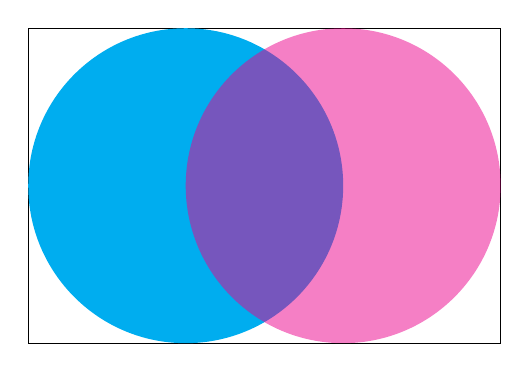
\begin{tikzpicture}
         \draw (-2,-2) rectangle (4,2);
         \fill[cyan] (0,0) circle (2);
         \fill[magenta,opacity=0.5] (2,0) circle ({2});
    \end{tikzpicture}%
     
    Opacity with Animation:\\
    \begin{animateinline}[controls]{30}%
    \multiframe{101}{i=0+1}{%
         \begin{tikzpicture}
             \draw (-2,-2) rectangle (4,2);
             \fill[cyan] (0,0) circle (2);
             \fill[magenta,opacity=0.5] (2,0) circle ({2*\i/100});
         \end{tikzpicture}%
    }%
    \end{animateinline}%
     
    \end{document}